\documentclass[runningheads]{llncs}

\usepackage{amssymb}
\usepackage{amsmath}
%% The amsthm package provides extended theorem environments

% \usepackage{amsthm}
% AM commented out because it clashes with proof, etc

%% The lineno packages adds line numbers. Start line numbering with
%% \begin{linenumbers}, end it with \end{linenumbers}. Or switch it on
%% for the whole article with \linenumbers.
\usepackage{lineno}

%% Use package enumitem to align enumeration and itemization
\usepackage{enumitem}
\usepackage{listings}
\usepackage{courier}           % for the courier font (optional)
\usepackage{multicol}          % for two equations side by side
\usepackage[justification=centering]{caption}
\usepackage[dvipsnames]{xcolor}
\usepackage{stmaryrd}
\usepackage{hyperref}
%\usepackage{cleveref}
\usepackage{hieroglf}
\usepackage{scalerel}
\usepackage{tikz}
\usepackage{pgfplots}
\usepackage[export]{adjustbox} % for subfigures
\usepackage{semantic}          % for mathlig


\hypersetup{ % play with these to change the look of hyperlinks
    colorlinks=true,
    linkcolor=black,
    filecolor=magenta,
    urlcolor=blue,
    citecolor=black
}

\newcommand{\coq}{\scalebox{.6}{\textpmhg{\Ha}}}
\newcommand{\p}[1]{\ensuremath{\mathsf{#1}}} % predicate font
\newcommand{\m}[1]{\ensuremath{\mathit{#1}}} % math font
\newcommand{\braces}[1]{\left\{\begin{array}{l@{}} #1 \end{array}\right\}}
\let\ramify\lightning
\newcommand{\sz}{\texttt{SIZE}}
\newcommand{\ifty}{\texttt{INF}}
\newcommand{\defeq}{\mathbin{\stackrel{\Delta}{=}}}
\usetikzlibrary{shadows}
\usetikzlibrary{arrows.meta, positioning, decorations.pathmorphing, fit, matrix}
\mathlig{/|}{\mathbin{\wedge}} % additive conjunction


% required by LNCS
\renewcommand\UrlFont{\color{blue}\rmfamily}

\colorlet{red}{red!80!black}
\colorlet{green}{green!50!black}

%% NEW COMMANDS =============================================

\lstdefinestyle{myStyle}{
%	language=Coq,
    keywords={Inductive,Require,Import,Definition,Fixpoint,match,with,end,let,in,fix},
	basicstyle=\normalfont\footnotesize\tt,
    keywordstyle=\color{green}, % Blue clashes with the cyan links. Change if you want.
	stepnumber=1,
	tabsize=2,
    numbers=none,
    numberstyle=\tiny,
    numbersep=5pt,
	showspaces=false,
    escapechar=`,
	showstringspaces=false
}
%basicstyle=\fontsize{10}{11}\selectfont\ttfamily,

\lstdefinestyle{myTinyStyle}{
%   language=Coq,
    basicstyle=\normalfont\fontsize{7.0}{7.3}\tt,
    keywordstyle=\color{green}, % Blue clashes with the cyan links. Change if you want.
    stepnumber=1,
    tabsize=2,
    numbers=none,
    numberstyle=\tiny,
    numbersep=5pt,
    showspaces=false,
    showstringspaces=false,
      language=C,
  morecomment=[l][{\color{OliveGreen}}]{//},
  sensitive=true,
  mathescape=true,
  showlines=true,
  escapechar=`,
  basicstyle=\footnotesize\ttfamily,
  keywordstyle=\color{blue}, numbers=left,
  numberstyle=\tiny, numbersep=5pt, boxpos=t
  }

\lstset{style=myTinyStyle}
\makeatletter
\newlength{\@mli}
\newcommand{\mli}[1]{%
  \settowidth{\@mli}{\lstinline/#1/}
  \hspace{-.5ex}\begin{minipage}[t]{\@mli}\lstinline/#1/\end{minipage}}
\makeatother
\newcommand{\li}[1]{\ifmmode\mbox{\mli{#1}}\else\mbox{\lstinline/#1/}\fi}

\newcommand\hide[1]{}

\newenvironment{centermath}
 {\begin{center}$\displaystyle}
 {$\end{center}}

\renewcommand{\note}[2][polish]{{\color{red} #2}{\marginpar{\tiny \color{blue} #1}}}
\renewcommand{\implies}{\Rightarrow}
\renewcommand{\iff}{\Leftrightarrow}

\title{A Machine-Checked C Implementation of Dijkstra's Shortest Path Algorithm}
\subtitle{(Short Paper)}
\titlerunning{A Machine-Checked C Implementation of Dijkstra's Shortest Path Algorithm}
%optional, please use if title is longer than one line

\begin{document}

\author{Anshuman Mohan$^{(\dagger)}$ \and Shengyi Wang$^{(\dagger)}$ \and Aquinas Hobor$^{(\dagger,\ddagger)}$}
\authorrunning{A. Mohan, S. Wang, A. Hobor}

%\author{Linh Tran \and Anshuman Mohan \and Aquinas Hobor}
%\authorrunning{L. Tran, A. Mohan, A. Hobor}
% First names are abbreviated in the running head.
% If there are more than two authors, 'et al.' is used.
%
\institute{($\dagger$) School of Computing and ($\ddagger$) Yale-NUS College, National University of Singapore}
% \\
% \email{\{hobor\}@comp.nus.edu.sg}}


\maketitle
%\begin{frontmatter}

%% Title, authors and addresses

%% use the tnoteref command within \title for footnotes;
%% use the tnotetext command for theassociated footnote;
%% use the fnref command within \author or \address for footnotes;
%% use the fntext command for theassociated footnote;
%% use the corref command within \author for corresponding author footnotes;
%% use the cortext command for theassociated footnote;
%% use the ead command for the email address,
%% and the form \ead[url] for the home page:

%% \tnotetext[label1]{}
%% \author{Name\corref{cor1}\fnref{label2}}
%% \ead{email address}
%% \ead[url]{home page}
%% \fntext[label2]{}
%% \cortext[cor1]{}
%% \address{Address\fnref{label3}}
%% \fntext[label3]{}

%% use optional labels to link authors explicitly to addresses:
%% \author[label1,label2]{}
%% \address[label1]{}
%% \address[label2]{}

%\author{}

%\address{}


\begin{abstract}
\vspace{-1.2em}
We report on a machine-checked Coq proof of correctness for
Dijkstra’s one-to-all shortest path algorithm.
We prove full functional correctness.
We use classic textbook code written in CompCert C, and since our
code is executable and realistic our verification
must deal with real-world complications.
In particular, we encounter and explain an overflow issue in
Dijkstra’s algorithm. The precise bound in the relevant precondition is
nontrivial: we show that the intuitive guess
fails and provide a workable refinement.
This work fits into an ongoing exploration of verified graph-manipulating
algorithms in a realistic setting.

\keywords{Dijkstra's shortest-path \and verification \and CompCert \and VST}
\end{abstract} %\and Coq 

%\end{frontmatter}

%% \linenumbers

%% main text

\section{Introduction}
\label{sec:intro}
Over the last fifteen years great strides have been made in automating verifications of programs that manipulate
tree-like data structures using separation logic 
\cite{berdine:smallfoot,chin:hipsleek,jacobs:verifast,chlipala:bedrock,bengtson:charge,appel:programlogics}.  Unfortunately, verifying programs that manipulate graph-like data structures (i.e. structures with \emph{intrinsic sharing}) has been more challenging.  Indeed, verifying such programs was formidable enough that a number of the early landmark results in separation logic devoted substantial effort to verify single examples such as Schorr-Waite~\cite{hongseok:phd} with pen and paper---avoiding the additional challenges inherent in mechanized reasoning.

In recent years, Hobor and Villard introduced the concept of \emph{ramification} as a kind of proof pattern or framework to verify graph-manipulating programs on pen and paper~\cite{hobor:ramification}.  The major focus of this paper is to develop methods to verify realistic graph programs in a mechanized context.  We do so by upgrading the theory of ramification and by developing a general and modular library for graph-related reasoning in separation logic.  We incorporate our approach into two sizeable separation logic-based verification tools: the Floyd system of the Verified Software Toolchain (VST)~\cite{appel:programlogics} and the HIP/SLEEK program verifier~\cite{chin:hipsleek}.  VST and HIP/SLEEK inhabit quite different points in the design space for verification tools, with VST primarily focused on heavily human-guided verifications with an emphasis on end-to-end machine-checked proofs, and HIP/SLEEK focusing on more automation.  Despite these differences, the vast majority of our Coq code base is shared between them,
giving us hope that our work will be applicable to other verification tools.

\marginpar{\color{magenta} computable mathgraphs, null, pregraphs Problem with ``later'' not being precise.}
The structure of our paper is as follows:
%\vspace{-0.25ex}
\begin{itemize}
\item[\S\ref{sec:orientation}] We verify a graph marking algorithm and explain why such algorithms are easier to verify using relations instead of functions.  We introduce \emph{localization blocks} as a new notation for ramification.  We upgrade Hobor and Villard's \infrulestyle{Ramify} rule to handle both modified program variables and existential quantifiers more gracefully.
\vspace{-0.1ex}
\item[\S\ref{sec:mathgraph}] We develop a general mechanization of mathematical graphs powerful enough to support realistic verification. %{\color{magenta} What else can we say here?}
\vspace{-0.1ex}
\item[\S\ref{sec:spacegraph}] We show that the standard Knaster-Tarski fixpoint~\cite{tarski:fixpoint} cannot define a usable separation logic graph predicate.  We propose a better definition for general spatial graphs that still enjoys a ``recursive'' fold/unfold.  We prove general theorems about spatial graphs in a way that can be utilized in multiple flavors of separation logic, such as the logics contained in VST and HIP/SLEEK.
\vspace{-0.1ex}
\item[\S\ref{vst}] We explain how we integrated ramification into VST by developing two new Floyd tactics, \li{localize} and \li{unlocalize}.  We discuss other examples we have verified, including spanning tree and DAG copy.
\vspace{-0.1ex}
\item[\S\ref{sec:hipsleek}] We explain how we modified HIP/SLEEK to introduce ramifications when programs modify data structures with intrinsic sharing and to automatically discharge the associated obligations using Coq-verified external lemmas.
\vspace{-0.1ex}
\item[\S\ref{sec:related}] We discuss related work, future work, and conclude.
\end{itemize}
All of our results are machine checked.



\section{Verified Dijkstra in C}
\label{sec:overview}

Figure~\ref{fig:decorated} shows the code and proof
sketch of Dijkstra's algorithm. 
The code is implemented exactly as suggested 
by~\cite{clrs}, and so we elide a discussion 
of the algorithm itself. The heart of the formal verification is in the 
while loop's invariant, which is stated on line~\ref{code:whileinv}
and explained further in Figure~\ref{fig:defns}.
The source vertex $\m{src}$ is taken as a parameter. 
A destination vertex $\m{dst}$ falls into one of three
categories, and subsequently obeys one of three invariants:
\begin{enumerate}
\item $\m{inv\_popped}$: $\m{dst}$ has been fully processed, and has been
popped from the priority queue. 
A globally optimal path from $\m{src}$ 
to $\m{dst}$ exists, the cost of this path is logged in 
the \texttt{dist} array, and all the vertices visited by the path are also popped.
Further, the links of this path are correctly logged in the \texttt{prev} array.
\item $\m{inv\_unpopped}$: $\m{dst}$ is reachable in 
one hop from a ``\emph{mom}'' vertex, which is itself popped. 
This route is locally optimal: we cannot 
improve the cost by going via a \emph{different} popped vertex.
The \texttt{prev} array logs
\emph{mom} as the best-known way to reach $\m{dst}$, and the \texttt{dist}
array logs the cost of the path via \emph{mom} as the best-known cost.
\item $\m{inv\_unseen}$: no path is currently known from $\m{src}$ to $\m{dst}$.
\end{enumerate}

This three-part invariant is trivially true before the while loop. 
On line~\ref{code:pop}, the minimal vertex from the priority queue is popped, 
thus breaking the invariant.

First, we must show that the minimal vertex $\m{u}$ 
obeys $\m{inv\_popped}$. \emph{i.e.}, show that the locally 
optimal path to $\m{u}$ is, in fact, globally optimal. 
This comes from blah blah blah

\newcommand{\s}{11}
\begin{figure}[htbp]
  \centering
  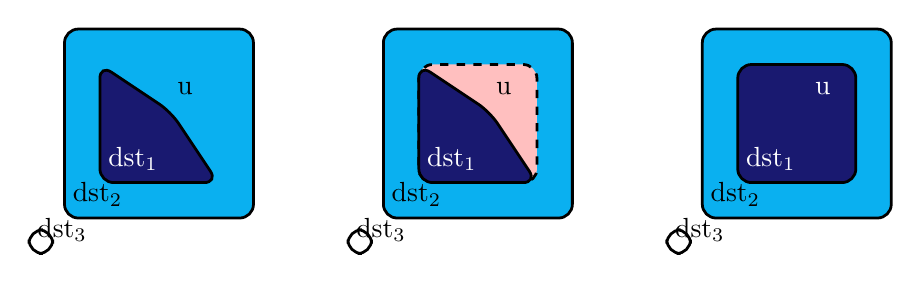
\begin{tikzpicture}[x=0.3cm, y=0.3cm,
      popped/.style={rounded corners=5pt, line width=1pt, draw, fill=MidnightBlue},
      fringe/.style={rounded corners=5pt, line width=1pt, draw, fill=ProcessBlue},
      popping/.style={rounded corners=5pt, line width=1pt, draw, dashed, fill=pink},
      unseen/.style={rounded corners=5pt, line width=1pt, draw}]
    \draw[unseen] (0,0) -- (\s,0) -- (\s,\s) -- (0,\s) -- cycle;
    \draw[fringe] (1.5,1.5) -- (9.5,1.5) -- (9.5,9.5) -- (1.5,9.5) -- cycle;
    \draw[popped] (3,3) -- (8,3) -- (6,6) -- (3,8) -- cycle;
    \node at (1.4,1) {dst$_3$};   
    \node at (2.9,2.5) {dst$_2$};   
    \node at (4.4,4) {\color{white}dst$_1$}; 
    \node at (6.6,7) {u};
    \tikzset{shift={(13.5,0)}}

    \draw[unseen] (0,0) -- (\s,0) -- (\s,\s) -- (0,\s) -- cycle;
    \draw[fringe] (1.5,1.5) -- (9.5,1.5) -- (9.5,9.5) -- (1.5,9.5) -- cycle;
    \draw[popping] (3,3) -- (8,3) -- (8,8) -- (3,8) -- cycle;
    \draw[popped] (3,3) -- (8,3) -- (6,6) -- (3,8) -- cycle;
    \node at (1.4,1) {dst$_3$};   
    \node at (2.9,2.5) {dst$_2$};   
    \node at (4.4,4) {\color{white}dst$_1$}; 
    \node at (6.6,7) {u};     

    \tikzset{shift={(13.5,0)}}

    \draw[unseen] (0,0) -- (\s,0) -- (\s,\s) -- (0,\s) -- cycle;
    \draw[fringe] (1.5,1.5) -- (9.5,1.5) -- (9.5,9.5) -- (1.5,9.5) -- cycle;
    \draw[popped] (3,3) -- (8,3) -- (8,8) -- (3,8) -- cycle;
    \node at (1.4,1) {dst$_3$};   
    \node at (2.9,2.5) {dst$_2$};   
    \node at (4.4,4) {\color{white}dst$_1$}; 
    \node at (6.6,7) {\color{white}u};       
  \end{tikzpicture}
  \caption{Popping $\m{u}$}  
\end{figure}

Next, we must account for the ripple effect that popping 
$\m{u}$ could have had on the other vertices. 
In particular, it is possible that a vertex obeying $\m{inv\_unpopped}$ can
improve its cost via $\m{u}$, and that an unreachable vertex 
obeying $\m{inv\_unseen}$ can now be reached via $\m{u}$. 
The for loop repairs these breakages by 
checking if a path via $\m{u}$ is an improvement for such vertices, and, if so, 
edits both arrays and the priority queue as seen on line~\ref{code:update}.

The for loop's invariant is similar to that of the while loop---$\m{inv\_unseen}$ 
and $\m{inv\_popped}$ are preserved as-is, modulo the popping of 
$\m{u}$ as discussed above. The key edit is in $\m{inv\_unpopped}$. blah blah blah

\colorlet{stash}{red}
\colorlet{red}{maincolor}

\begin{lstlisting}
  void dijkstra (int graph[SIZE][SIZE], int src, 
                           int *dist, int *prev) {
$//$ $\braces{\p{DijkGraph}(\gamma)}$
    int pq[SIZE];
    int i, j, u, cost;
    for (i = 0; i < SIZE; i++) {
      dist[i] = INF; 
      prev[i] = INF; 
      pq[i] = INF;
    }
    dist[src] = 0; 
    pq[src] = 0; 
    prev[src] = src;
$//$ $\braces{\p{DijkGraph}(\gamma) /| \null \\
\m{dijk\_correct}(\gamma,\m{src},\m{prev},\m{dist},\m{priq})}$
    while (!pq_emp(pq)) {
      u = popMin(pq);
      for (i = 0; i < SIZE; i++) {
        cost = graph[u][i]; 
        if (cost < INF) {
          if (dist[i] > dist[u] + cost) {
            dist[i] = dist[u] + cost;
            prev[i] = u; 
            pq[i] = dist[i];
          }
        }  
      }
    }
$//$ $\braces{\p{DijkGraph}(\gamma) /| \null \\ 
\forall \m{dst} \in \m{priq}.~\m{priq}[\m{dst}] = \texttt{INF} /| \null \\ 
\m{dijk\_correct}(\gamma,\m{src},\m{prev},\m{dist},\m{priq})}$
    return;
  }
\end{lstlisting}
\vspace{0.5em}
\begin{equation*}
\begin{split}
\p{list\_rep}(\gamma, \m{i}) &\defeq \texttt{data\_at  array  graph2mat}(\gamma)[\m{i}] \texttt{  list\_addr}(\gamma, \m{i}) \\
\vspace{1em}
\p{graph\_rep}(\gamma) &\defeq \underset{\texttt{vvalid}(\gamma,\m{v})}{\bigstar} \m{v}  \mapsto\p{list\_rep}(\gamma, \m{v})
\end{split}
\end{equation*}

\begin{equation*}
\begin{split}
\m{dijk\_correct}(\gamma, \m{src}, \m{prev}, \m{dist},& \m{priq}) \; \defeq \; \\
\forall \m{dst}.~\m{dst} \in \m{popped}(\m{priq}) \; => \; & \exists \m{path}.~\m{path\_correct}(\gamma, \m{prev}, \m{dist}, \m{path}) /| \null \\
& \m{path\_glob\_optimal}(\gamma, \m{dist}, \m{path}) /| \null \\
& \m{path\_entirely\_in\_popped}(\gamma, \m{prev}, \m{path}) /| \null \\
\m{priq}[\m{dst}] < \ifty \; => \; & \texttt{let }\m{m} \texttt{ := } \m{prev}[\m{dst}] \texttt{ in } \m{m} \in \m{popped}(\m{priq}) /| \null \\
&\forall \m{m'} \in \m{popped}(\m{priq}).~\m{cost}(\m{path2m} +:: (m, dst)) \le \null \\
&\hspace{10em} \m{cost}(\m{path2m'} +:: (m', dst)) /| \null \\
\m{priq}[\m{dst}] = \ifty \; => \; & \forall \m{m} \in \m{popped}(\m{priq}).~\m{cost}(\m{path2m} +:: (m, dst)) = \ifty
\end{split}
\end{equation*}

\colorlet{red}{stash}




\section{I'm sorry Dave, I'm afraid I can't do that: Overflow}
\label{sec:overflow}
Dijkstra's algorithm clearly cannot work when a path
cost is more than \texttt{INT\_MAX}.  A reasonable-looking restriction
is to bound edge costs by
$\left\lfloor\frac{\texttt{INT\_MAX}}{\texttt{size}-1}\right\rfloor$, since
the longest optimal path has $\texttt{size}-1$ links and so the
most expensive possible path costs no more than \texttt{INT\_MAX}.
However, this has two flaws.  First, since we are writing real code in~C,
rather than pseudocode in an idealized setting, we must reserve some
concrete \texttt{int} value \texttt{inf} for ``infinity'', with 
the semantics that if the best-known distance to a vertex~\m{x}
is \texttt{inf}, then~\m{x} is as-yet unreachable.
A consequence of this is that reachable destination vertices cannot have a
path cost of \texttt{inf}: if they did, this would be logged in the
\texttt{dist} array and create an ambiguity.
Second, even though the best-known distances start at \texttt{inf}
(see line~\ref{code:assigninf}) and only ever decrease from there, the code can
overflow on lines~\ref{code:overflow}~and~\ref{code:update1}.

\begin{figure}[t]
\centering
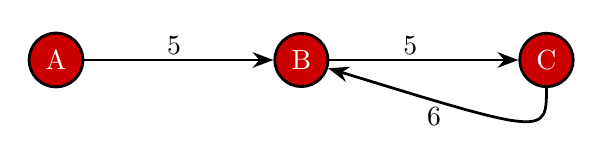
\begin{tikzpicture}[x=0.3cm, y=0.3cm,
  vert/.style={circle, line width=1pt, draw, fill=red}]
  \node[vert] (A) at (0,0) {\color{white}A};
  \node[vert] (B) [right = 8 of A] {\color{white}B};
  \node[vert] (C) [right = 8 of B] {\color{white}C};
  \draw [->,line width=1pt,arrows={-Stealth}] (A) -- (B);
  \draw [->,line width=1pt,arrows={-Stealth}] (B) -- (C);
  \draw [->,line width=1pt,arrows={-Stealth}] (C.south) .. controls ++(0, -2) .. (B);
  \node at (5,0.6) {5};
  \node at (15,0.6) {5};
  \node at (16,-2.4) {6};
\end{tikzpicture}
\caption{A graph that will result in overflow on a 4-bit machine.}
\label{fig:overflow}
\end{figure}

Consider applying Dijkstra's algorithm on a hypothetical 4-bit unsigned machine to
the graph in figure~\ref{fig:overflow}.  The \texttt{size} of the graph is 3 nodes, and so the na\"ive edge-weight upper bound is $\left\lfloor\frac{\texttt{INT\_MAX}}{\texttt{size}-1}\right\rfloor = \left\lfloor\frac{15}{3-1}\right\rfloor = 7$, for example as in the graph pictured in figure~\ref{fig:overflow}.  Indeed, a glance at the figure is enough to tell that the true distance from the source~A~to vertices~B~and~C~are~5~and~10 respectively---both of which are representable with 4 bits, and so na\"ively all seems well.  %Unfortunately, Dijkstra's algorithm does not exactly work like that.
Indeed, after processing vertices~A~and~B, 5~and~10~\emph{are} the costs reflected in the \texttt{dist} array for~B~and~C respectively---\emph{but unfortunately vertex~C~is still in the priority queue}.  After vertex~C~is popped on line~\ref{code:pop}, we fetch its neighbors in the \texttt{for} loop; the cost from C~to~B~(6)~is fetched on line~\ref{code:cost}.  On line~\ref{code:overflow} the currently optimal cost to~B~(5) is compared with the sum of the optimal cost to~C~(10) plus the just-retrieved cost of the edge from~C~to~B~(6).  Since $10+6$ overflows in 4-bit arithmetic, the comparison is not between~5~and~16 but in fact between~5~and~0!  Thus the code decides that a new cheaper path from~A~to~B~exists (in particular, A$\leadsto$B$\leadsto$C$\leadsto$B) and then trashes the \texttt{dist} and \texttt{prev} arrays on line~\ref{code:update1}.

Our code uses signed \texttt{int} rather than \texttt{unsigned int} so we have undefined behavior rather than defined-but-wrong behavior, but the essence of the overflow is identical.
Our solution is twofold.  First, we restrict the maximum edge cost to $\left\lfloor\frac{\texttt{INT\_MAX}}{\texttt{size}}\right\rfloor - 1$, which in the 4-bit setting just described forces an edge cost of no more than~4.  Consider modifying figure~\ref{fig:overflow} to
have edge weights of~4~rather than~5s~and~6s.  After processing vertices~A~and~B, the distances to~B~and~C are no more than~4~and~8 respectively.  When we process vertex~C, the comparison on line~\ref{code:overflow} is thus between the previous best cost to~B~(4) and the candidate best cost to~B~via~C~(12); there is no overflow and the code behaves as advertised.

The second part of our solution is that we require in the function precondition that $\left\lfloor \frac{\texttt{INT\_MAX}}{\texttt{size}} \right\rfloor - 1 < \texttt{inf} \le \texttt{INT\_MAX} - \left\lfloor \frac{\texttt{INT\_MAX}}{\texttt{size}} \right\rfloor + 1$.  As long as $\texttt{size} > 1$, this is perfectly realizable  by setting \texttt{inf} to $\texttt{INT\_MAX} - \left\lfloor \frac{\texttt{INT\_MAX}}{\texttt{size}} \right\rfloor + 1$, \emph{i.e.} in the 4-bit machine we set \texttt{inf} to $11$.  When $\texttt{size} = 1$, this inequality is not realizable; our verification is thus not applicable to single-vertex graphs, a special case for which the shortest-path problem is in any event rather uninteresting.



%% If you have bibdatabase file and want bibtex to generate the
%% bibitems, please use
%%
%\bibliographystyle{plainurl}% the mandatory bibstyle

\section{Concluding thoughts: Future and Related Work}
\label{sec:conclusion}
\subsection{Related work}

We have already discussed work directly related Dijkstra's (\S\ref{sec:relworkdijkstra}), Prim's (\S\ref{sec:relworkprim}), and Kruskal's (\S\ref{sec:relworkkruskal}) algorithms in detail, including work from both the algorithms and formal methods literature.  Briefly to the point of unreasonableness, our observations about Dijkstra's overflow and Prim's specification are novel, and existing formal proofs focus on code working within idealized environments rather than handling the real-world considerations that we do.  We have also already discussed the three formal developments we
build upon and extend: CompCert, VST, and CertiGraph (\S\ref{sec:stats}).  Our goal now is to discuss mechanized graph reasoning and verification more broadly.

\paragraph{Reasoning about mathematical graphs.}
There is a 30+ year history of mechanizing graph theory, beginning at least with Wong~\cite{wong1991} and Chou~\cite{chou1994formal} and continuing to the present day; Wang discusses many such efforts~\cite[\S3.3]{shengyi:thesis}.  The two abstract frameworks that seem closest to ours are those by Noschinski~\cite{Noschinski2015}; and by Lammich and Nipkow~\cite{DBLP:journals/afp/LammichN19}.  The latter is particularly relevant to our work, because they too start with a directed graph library and must extend it to handle undirected graphs so that they can verify Prim's algorithm.

\paragraph{More-automated verification.}
Broadly speaking, mechanized verification of software falls in a spectrum between more-automated-but-less-precise verifications and less-automated-but-more-precise verifications.  Although VST contains some automation, we fall within the latter camp.  In the former camp, landmark initial separation logic~\cite{o2001local} tools such as Smallfoot~\cite{berdine:smallfoot} have grown into Facebook's industrial-strength Infer~\cite{calcagno2015moving}.  Other notable relatively-automated separation logic-based tools include HIP/SLEEK~\cite{chin:hipsleek}, Bedrock~\cite{chlipala:bedrock}, and VerCors~\cite{DBLP:conf/fm/BlomH14}.  Boogie~\cite{barnett2005boogie}, \textsc{Blast}~\cite{DBLP:journals/sttt/BeyerHJM07}, Dafny~\cite{leino10}, and KeY~\cite{DBLP:series/lncs/10001} are examples of more-automated solutions that do not use separation logic.  In \S\ref{sec:relworkdijkstra} we discuss how some of these more-automated approaches have been applied to verify Dijkstra's algorithm. Petrank and Hawblitzel's Boogie-based verification of a garbage collector~\cite{gcexample2} gives another more-automated verification of a graph algorithm.

We are not confident that more-automated tools would be able to replicate our work easily.  We prove full functional correctness, whereas many more-automated tools prove only more limited properties.  Moreover, our full functional correctness results rely upon a meaningful amount of domain-specific knowledge about graphs, which automated tools usually lack.  Even if we restrict ourselves to more limited domains such as overflows, several more automated efforts did not uncover the overflow we did (\S\ref{sec:relworkdijkstra}).  The proof that certain bounds on edge weights and \texttt{inf} suffice depends on an intimate understanding of Dijkstra's algorithm (in particular, that it explores one edge beyond the optimum paths); overall the problem seems challenging in highly-automated settings.  The more powerful specification we discover for Prim's algorithm in \S\ref{sec:primforest} is likewise not something a tool is likely to discover: human insight appears necessary, at least given the current state of machine learning techniques.

In contrast, several of the potential overflows in our binary heap might be uncovered by more-automated approaches, especially those related to the \texttt{PARENT} and \texttt{LEFT\_CHILD} macros from \S\ref{sec:heapinsertremove}.  Although the arithmetic involves both addition/subtraction and multiplication/division, we suspect a tool such as Z3~\cite{moura2008} could handle it. \hide{; the multiplication/division always has the constant \texttt{2u} for an operand.}  Moreover, a sufficiently-precise tool would probably spot the necessity of forcing the internal constants into \texttt{unsigned int}.  The issue of sound key generation described in~\S\ref{sec:modpri} might be a bit trickier.  On the one hand, \texttt{unsigned int} overflow is defined in~C, so real code sometimes relies upon it.  Accordingly, merely observing that the counter could overflow does not guarantee that the code is necessarily buggy.  On the other hand, some tools might flag it anyway out of caution (\emph{i.e.} right answer, wrong reason).

\paragraph{Less-automated verification.}
Although as discussed above some more-automated tools have been applied to verify graph algorithms, the problem domain is sufficiently complex that many of the verifications discussed in \S\ref{sec:relworkdijkstra}, \S\ref{sec:relworkprim}, and \S\ref{sec:relworkkruskal} use less-automated techniques.  Two basic approaches are popular.  Approach A: write the algorithm in the native language of a proof assistant and then use tactics to reason about it.  Approach B: write the algorithm in another language with a precisely defined semantics, and then use tactics to reason about it.  We take approach B due to our use of VST; one of VST's more popular competitors in this style is ``Iris Proof Mode''~\cite{DBLP:conf/popl/KrebbersTB17}.  In contrast, Lammich \emph{et al.} have produced a series results verifying a variety of graph algorithms that generally take approach A~\cite{DBLP:conf/itp/Lammich14,DBLP:journals/afp/LammichN19,DBLP:journals/afp/HaslbeckLB19,cite,cite,cite}.  Lammich has also verified

%dijkstra_shortest_path-afp

Generally speaking, the most comprehensive work on v


other authors less push-button approaches are still popular.

\paragraph{Verifying graph algorithms}



%\note{Being in pseudocode and , these works do not need to discuss the application of the algorithms on "strange", non-simple graph inputs. Our C implementation does account for such inputs to a small extent, such as the edge list containing multiple edges between two vertices in Kruskal's.}

\paragraph{Other graph proof libraries.} Krishna et al~\cite{DBLP:conf/esop/KrishnaSW20} has developed a flow algebraic framework to reason about local and global properties of \textit{flow graphs} in the program heap. Their flow algebra is designed to mainly tackle local reasoning of global graphs in program heaps, tackling similar issues to Wang et al ~\cite{DBLP:journals/pacmpl/WangCMH19}, but in this paper, local reasoning is not required. Their flow algebra is said to be compatible with existing separation logics, although actual implementation and integration with SL tools appears to be an ongoing progress.
%In a related vein, Paulin and Filli\^atre verified Floyd's algorithm in Coq~\cite{paulin}

\subsection{Previous work} We have long been interested in
the verification of graph-manipulating programs written in~C~\cite{hobor:ramification}.
We fortified our techniques to handle realistic (CompCert~\cite{leroy:compcert})~C~to a machine-checked level of rigour~\cite{DBLP:journals/pacmpl/WangCMH19}.  Novel features of the present result include a previously-untried adjacency matrices spatial graph representation as well as non-trivial edge labels between graph nodes. % for the first time. %, used to represent cost. %; both are new for us.

\subsection{Ongoing and future work}
{\color{red}We are investigating techniques to increase the automation of such verifications.  Although
we benefit from some automation at the Hoare-logic level provided by the Verified Software
Toolchain~\cite{appel:programlogics}, building these proofs is still highly labor intensive.  We see potential
for automation in four areas: (A) the Hoare level; (B) the spatial level; (C) the mathematical level; and (D) the interface between the spatial and the mathematical levels.  Our ongoing work
on these challenges include (A) improved tactics for VST for common cases we encounter in graph
algorithms; (B) an expanded library of existing graph constructions such as the adjacency-matrix representation used in this result, as well as associated lemmas;
(C) better lemmas about common mathematical graph patterns, investigations into reachability techniques
based on regular expressions over matrices and related semirings~\cite{backhouse,DBLP:journals/jacm/Tarjan81a,dolan2013fun,krishna2017go}; and (D) improved modularity in our constructions and
automation of common cases, \emph{e.g.} we often compare~C~pointers to heap-represented graph
nodes for equality, and due to the nature of our representations this equality check will be
well-defined in~C~when the associated nodes are present in the mathematical graph.  The key
advantage of having end-to-end machine-checked examples such as the one we presented above is
that they guide the automation efforts by providing precise goals that are known to be strong
enough to verify real code.}

%@misc{paulin,
%title={The {C}oq proof assistant},
%author={{C}oq development team},
%url={https://coq.inria.fr/}, journal={The Coq Proof Assistant}}
%C. and J.C. Filli\^atre
%http://pauillac.inria.fr/cdrom/www/coq/contribs/floyd.html
%.11. R.Sumners.Corre
%tne


\hide{
\paragraph{Conclusion.}
We described a machine-checked proof of correctness for Dijkstra’s
shortest-path algorithm written in real~C from classic textbook code.
We showed this code suffers from an overflow bug and described a precise
precondition on edge weights to avoid it.  We put this result
in the context of our ongoing work.
} 

\bibliographystyle{splncs}
\bibliography{dijkstra}

%% The Appendices part is started with the command \appendix;
%% appendix sections are then done as normal sections
\appendix
\label{sec:apx}

Explain how the previous observations plug into Wang '19

Explain dijkstra\_correct, the correctness condition on the while loop

Explain that by the time the loop ends, we'll be done

Use annotated proof:

\colorlet{stash}{red}
\colorlet{red}{maincolor}

\begin{lstlisting}
  void dijkstra (int graph[SIZE][SIZE], int src, 
                           int *dist, int *prev) {
$//$ $\braces{\p{DijkGraph}(\gamma)}$
    int pq[SIZE];
    int i, j, u, cost;
    for (i = 0; i < SIZE; i++) {
      dist[i] = INF; 
      prev[i] = INF; 
      pq[i] = INF;
    }
    dist[src] = 0; 
    pq[src] = 0; 
    prev[src] = src;
$//$ $\braces{\p{DijkGraph}(\gamma) /| \null \\
\m{dijk\_correct}(\gamma,\m{src},\m{prev},\m{dist},\m{priq})}$
    while (!pq_emp(pq)) {
      u = popMin(pq);
      for (i = 0; i < SIZE; i++) {
        cost = graph[u][i]; 
        if (cost < INF) {
          if (dist[i] > dist[u] + cost) {
            dist[i] = dist[u] + cost;
            prev[i] = u; 
            pq[i] = dist[i];
          }
        }  
      }
    }
$//$ $\braces{\p{DijkGraph}(\gamma) /| \null \\ 
\forall \m{dst} \in \m{priq}.~\m{priq}[\m{dst}] = \texttt{INF} /| \null \\ 
\m{dijk\_correct}(\gamma,\m{src},\m{prev},\m{dist},\m{priq})}$
    return;
  }
\end{lstlisting}
\vspace{0.5em}
\begin{equation*}
\begin{split}
\p{list\_rep}(\gamma, \m{i}) &\defeq \texttt{data\_at  array  graph2mat}(\gamma)[\m{i}] \texttt{  list\_addr}(\gamma, \m{i}) \\
\vspace{1em}
\p{graph\_rep}(\gamma) &\defeq \underset{\texttt{vvalid}(\gamma,\m{v})}{\bigstar} \m{v}  \mapsto\p{list\_rep}(\gamma, \m{v})
\end{split}
\end{equation*}

\begin{equation*}
\begin{split}
\m{dijk\_correct}(\gamma, \m{src}, \m{prev}, \m{dist},& \m{priq}) \; \defeq \; \\
\forall \m{dst}.~\m{dst} \in \m{popped}(\m{priq}) \; => \; & \exists \m{path}.~\m{path\_correct}(\gamma, \m{prev}, \m{dist}, \m{path}) /| \null \\
& \m{path\_glob\_optimal}(\gamma, \m{dist}, \m{path}) /| \null \\
& \m{path\_entirely\_in\_popped}(\gamma, \m{prev}, \m{path}) /| \null \\
\m{priq}[\m{dst}] < \ifty \; => \; & \texttt{let }\m{m} \texttt{ := } \m{prev}[\m{dst}] \texttt{ in } \m{m} \in \m{popped}(\m{priq}) /| \null \\
&\forall \m{m'} \in \m{popped}(\m{priq}).~\m{cost}(\m{path2m} +:: (m, dst)) \le \null \\
&\hspace{10em} \m{cost}(\m{path2m'} +:: (m', dst)) /| \null \\
\m{priq}[\m{dst}] = \ifty \; => \; & \forall \m{m} \in \m{popped}(\m{priq}).~\m{cost}(\m{path2m} +:: (m, dst)) = \ifty
\end{split}
\end{equation*}

\colorlet{red}{stash}


\begin{equation*}
\begin{split}
\p{list\_rep}(\gamma, \m{i}) &\defeq \texttt{data\_at  array  graph2mat}(\gamma)[\m{i}] \texttt{  list\_addr}(\gamma, \m{i}) \\
\vspace{1em}
\p{graph\_rep}(\gamma) &\defeq \underset{\texttt{vvalid}(\gamma,\m{v})}{\bigstar} \m{v}  \mapsto\p{list\_rep}(\gamma, \m{v})
\end{split}
\end{equation*}

\begin{equation*}
\begin{split}
&\!\!\!\!\!\!\m{path\_correct}(\gamma, \m{src}, \m{prev}, \m{dist}, \m{mom}, \m{p}) \; \defeq \; 
\m{valid\_path}(\gamma, \m{p}) /| \m{path\_ends}(\gamma, \m{p}, \m{src}, \m{dst}) /| \null \\
&\m{path\_cost}(\gamma, \m{p}) \not= \texttt{INF} /| \m{dist}[\m{dst}] = \m{path\_cost}(\gamma, \m{p}) /| \forall \m{a, b}.~\m(a,b) \in p -> \m{prev}[\m{b}] = \m{a} \\
\vspace{2em}
&\!\!\!\!\!\!\m{path\_globally\_optimal}(\gamma, \m{src}, \m{dst}, \m{p}) \; \defeq \; 
\forall \m{p'}.~\m{valid\_path}(\gamma, \m{p'}) -> \m{path\_ends}(\gamma, \m{p'}, \m{src}, \m{dst}) -> \\
&\hspace{20em}\m{path\_cost}(\gamma, \m{p}) \le \m{path\_cost}(\gamma, \m{p'}) \\
&\!\!\!\!\!\!\m{all\_hops\_in\_popped}(\m{p}, \m{priq}) \; \defeq \; 
\forall \m{a, b}.~\m{(a, b)} \in \m{p} -> \m{a} \in \m{popped}(\m{priq}) /| \m{b} \in \m{popped}(\m{priq})\\
&\!\!\!\!\!\!\m{all\_hops\_in\_popped\_weak}(\m{p}, \m{priq}, \texttt{u}) \; \defeq \; 
\forall \m{a, b}.~\m{(a, b)} \in \m{p} -> \m{a} \in \m{popped}(\m{priq}) /| \null \\ 
&\hspace{20em}\m{b} \in \m{popped}(\m{priq}) /| \m{a} \not= \texttt{u} /| \m{b} \not= \texttt{u} \\
\vspace{4em}
&\!\!\!\!\!\!\m{dijk\_correct}(\gamma, \m{src}, \m{prev}, \m{dist}, \m{priq}) \; \defeq \; \\
&\forall \m{dst}.~\texttt{0} \le \m{dst} < \texttt{SIZE} -> \m{inv\_popped}(\gamma, \m{src}, \m{prev}, \m{dist}, \m{priq}, \m{dst}) /| \null \\
&\hspace{11em}\m{inv\_unpopped}(\gamma, \m{src}, \m{prev}, \m{dist}, \m{priq}, \m{dst}) /| \null \\
&\hspace{11em}\m{inv\_unseen}(\gamma, \m{prev}, \m{dist}, \m{priq}, \m{dst}) \\
\vspace{1em}
&\!\!\!\!\!\!\m{dijk\_correct\_weak}(\gamma, \m{src}, \m{prev}, \m{dist}, \m{priq}, \texttt{i}, \texttt{u}, \texttt{SIZE}) \; \defeq \; \\
&\forall \m{dst}.~\texttt{0} \le \m{dst} < \texttt{SIZE} -> \m{inv\_popped}(\gamma, \m{src}, \m{prev}, \m{dist}, \m{priq}, \m{dst}) /| \null \\
&\hspace{11em}\m{inv\_unseen}(\gamma, \m{prev}, \m{dist}, \m{priq}, \m{dst}) /| \null \\
&\forall \m{dst}.~\texttt{0} \le \m{dst} < \texttt{i} -> \m{inv\_unpopped}(\gamma, \m{src}, \m{prev}, \m{dist}, \m{priq}, \m{dst}) /| \null \\
&\forall \m{dst}.~\texttt{i} \le \m{dst} < \texttt{SIZE} -> \m{inv\_unpopped\_weak}(\gamma, \m{src}, \m{prev}, \m{dist}, \m{priq}, \m{dst}, \texttt{u}) \\
\vspace{1em}
&\!\!\!\!\!\!\m{inv\_popped}(\gamma, \m{src}, \m{prev}, \m{dist}, \m{priq}, \m{dst}) \; \defeq \; \m{dst} \in \m{popped}(\m{priq}) -> \\
&\exists \m{p2dst}.~\m{path\_correct}(\gamma, \m{src}, \m{prev}, \m{dist}, \m{dst}, \m{p2dst}) /| \null \\
&\m{all\_hops\_in\_popped}(\m{p2dst}, \m{priq}) /|
\m{path\_globally\_optimal}(\gamma, \m{src}, \m{dst}, \m{p2dst}) \\
\vspace{1em}
&\!\!\!\!\!\!\m{inv\_unpopped}(\gamma, \m{src}, \m{prev}, \m{dist}, \m{priq}, \m{dst}) \; \defeq \; \m{priq}[\m{dst}] < \texttt{INF} -> \\
&\texttt{let } \m{mom} \texttt{ := } \m{prev}[\m{dst}] \texttt{ in } \exists \m{p2mom}.~\m{path\_correct}(\gamma, \m{src}, \m{prev}, \m{dist}, \m{mom}, \m{p2mom}) /| \null \\
&\m{all\_hops\_in\_popped}(\m{p2mom}, \m{priq}) /| \m{path\_globally\_optimal}(\gamma, \m{src}, \m{mom}, \m{p2mom}) /| \null \\
&\forall \m{mom', p2mom'}.~~\m{path\_correct}(\gamma, \m{src}, \m{prev}, \m{dist}, \m{mom'}, \m{p2mom'}) -> \\
&\m{all\_hops\_in\_popped}(\m{p2mom'}, \m{priq}) -> 
\m{path\_globally\_optimal}(\gamma, \m{src}, \m{mom'}, \m{p2mom'}) -> \\
&\m{path\_cost}(\m{p2mom} + \m{(mom, dst)}) \le \m{path\_cost}(\m{p2mom'} + \m{(mom', dst)}) \\
\vspace{1em}
&\!\!\!\!\!\!\m{inv\_unpopped\_weak}(\gamma, \m{src}, \m{prev}, \m{dist}, \m{priq}, \m{dst}) \; \defeq \; \m{priq}[\m{dst}] < \texttt{INF} -> \\
&\texttt{let } \m{mom} \texttt{ := } \m{prev}[\m{dst}] \texttt{ in } \exists \m{p2mom}.~\m{path\_correct}(\gamma, \m{src}, \m{prev}, \m{dist}, \m{mom}, \m{p2mom}) /| \null \\
&\m{all\_hops\_in\_popped\_weak}(\m{p2mom}, \m{priq}) /| \m{path\_globally\_optimal}(\gamma, \m{src}, \m{mom}, \m{p2mom}) /| \null \\
&\forall \m{mom', p2mom'}.~~\m{path\_correct}(\gamma, \m{src}, \m{prev}, \m{dist}, \m{mom'}, \m{p2mom'}) -> \\
&\m{all\_hops\_in\_popped\_weak}(\m{p2mom'}, \m{priq}) -> 
\m{path\_globally\_optimal}(\gamma, \m{src}, \m{mom'}, \m{p2mom'}) -> \\
&\m{path\_cost}(\m{p2mom} + \m{(mom, dst)}) \le \m{path\_cost}(\m{p2mom'} + \m{(mom', dst)}) \\
\vspace{1em}
&\!\!\!\!\!\!\m{inv\_unseen}(\gamma, \m{prev}, \m{dist}, \m{priq}, \m{dst}) \; \defeq \; \m{priq}[\m{dst}] = \texttt{INF} ->
(\m{dist}[\m{dst}] = \texttt{INF} /| \m{prev}[\m{dst}] = \texttt{INF})
\end{split}  
\end{equation*}
% 
\appendix

\section{Junk}
{\color{magenta} Universally-quantified metavariables can appear free in the predicates to make further connections.
Assuming that the abstracted pre- and postconditions $A$, $B$, $C$, and $D$ above all use \li{x}, we proceed
as follows.  First we introduce a new fresh metavariable $x$ whose value will be equal to \li{x} after the localization, and then choose $F \stackrel{\Delta}{=} [\li{x} |-> x] (C -* D)$, that is we substitute the program
variable \li{x} for the metavariable $x$.  Since we have substituted away \li{x}, $F$ ignores it and so we satisfy the side condition on \infrulestyle{Solve Ramify-P}.  We then must strengthen $C$ into $C' \stackrel{\Delta}{=} C /| \li{x} = x$ to make the connection at the appropriate program point.  Now we are left with the entailments
\[
\begin{array}{lcl}
\li{x} = 5 /| A & |- & (\li{x} = 5 /| B) * F \\
F & |- & (\li{x} = 6 /| C') -* (x = 6 /| D)
\end{array}
\]
To further relate the earlier and later values of \li{x} in $F$ we can introduce a second fresh $x'$ and use $B' \stackrel{\Delta}{=} B /| \li{x} = x'$.
}


\section{Remaining proof of \infrulestyle{Ramify-PQ}}
\label{apx}

See figure \ref{fig:remainrampq}.

\begin{figure*}[t]
\[
\infrule{}
{
  L_1 |- L_1 \\
  \infrule{}
  {
    \infrule{}
    {
      \infrule{}
      {
        \infrule{}
        {
          \infrule{}
          {
            \infrule{}
            {
              \infrule{}
              {
                \infrule{}
                {
                  \infrule{}
                  {
                    \infrule{}
                    {
                      [x |-> x_0] (L_2 -* G_2) |- [x |-> x_0](L_2 -* G_2)
                    } {
                      \forall x.~ (L_2 -* G_2) |- [x |-> x_0](L_2 -* G_2)
                    } {\forall \mathsf{e}}
                  } {
                    \forall x.~ (L_2 -* G_2) |- ([x |-> x_0]L_2) -* ([x |-> x_0]G_2)
                  } {\textrm{substitute}}
                } {
                  \big(\forall x.~ (L_2 -* G_2)\big) * [x |-> x_0]L_2 |- [x |-> x_0]G_2
                } {(3)}
              } {
                \big(\forall x.~ (L_2 -* G_2)\big) * [x |-> x_0]L_2 |- \exists x.~ G_2
              } {\exists \mathsf{i}}
            } {
            \big(\forall x.~ (L_2 -* G_2)\big) * (\exists x.~ L_2) |- \exists x.~ G_2
            } {\exists \mathsf{e}}
          } {
            \forall x.~ (L_2 -* G_2) |- (\exists x.~ L_2) -* (\exists x.~ G_2)
          } {(3)}
        } {
          |- \big(\forall x.~ (L_2 -* G_2)\big) => \big((\exists x.~ L_2) -* (\exists x.~ G_2)\big)
        } {=> \mathsf{i}}
      } {
        |- \pguards{c}\Big(\big(\forall x.~ (L_2 -* G_2)\big) => \big((\exists x.~ L_2) -* (\exists x.~ G_2)\big)\Big)
      } {\mathsf{N}}
    } {
      |- \Big(\pguards{c}\big(\forall x.~ (L_2 -* G_2)\big) \Big) => \Big( \pguards{c}\big((\exists x.~ L_2) -* (\exists x.~ G_2)\big) \Big)
    } {\mathsf{K}}
  } {
    \pguards{c}\big(\forall x.~ (L_2 -* G_2)\big) |- \pguards{c}\big((\exists x.~ L_2) -* (\exists x.~ G_2)\big)
  } {\mathsf{i} =>}
} {
  L_1 * \pguards{c}\big(\forall x.~ (L_2 -* G_2)\big) |- L_1 * \pguards{c}\big((\exists x.~ L_2) -* (\exists x.~ G_2)\big)
} {* \textrm{ split} }
\]
\caption{Remaining proof of \infrulestyle{Ramify-PQ}}
\label{fig:remainrampq}
\end{figure*}



%%\end{thebibliography}
\end{document}
\endinput
%%
